%===================================
%===================================
%===================================
\setchapterpreamble[u]{\margintoc}
\chapter{Combined cooling pilot plant at Plataforma Solar de Almería}
\labch{cc:facility}

\tldrbox{ In this chapter a detailed description of the combined cooling pilot
    plant at \gls{psaLabel} is provided including a \gls{pYidLabel} diagram and
    the methodology followed to perform the experimentation and data-processing.
    Several experimental campaigns have been performed to characterize the
    different components of the pilot plant and the complete system, at a wide
    range of operating conditions. Combined, 198 tests are processed most of
    which are openly available in public repositories. }

\section*{Introduction}

The combined cooling pilot plant at \fullgls{psaLabel} ---see
\reffig{cc:facility:cc-pilot-plant-diagram}--- is a unique facility that
integrates a wet cooling tower and a dry cooler\sidenote{Both provided by
\textit{Hamon D'Hondt}} in a flexible hydraulic configuration. It allows for the
study and validation of different cooling configurations, models, and control
and optimization strategies.
% Historia de la planta
The pilot plant was installed at \gls{psaLabel} in June 2019 as part of the
\textit{WASCOP} project (\textit{Water Saving for Solar Concentrated Power}),
within the Horizon 2020 (H2020) program. The main goal of the project was the
development of innovative technologies for water management in \gls{cspLabel}
plants.

This chapter describes the plant in \nrefsec{cc:facility:description} and the
experimental campaigns carried out in \nrefsec{cc:facility:exp}.

% TODO: A la salida de la segunda válvula hay que añadir una flecha para que
% sea más legible, renombrar válvulas V1 y V2 a Vp y Vs.
\begin{figure*}[h!]
	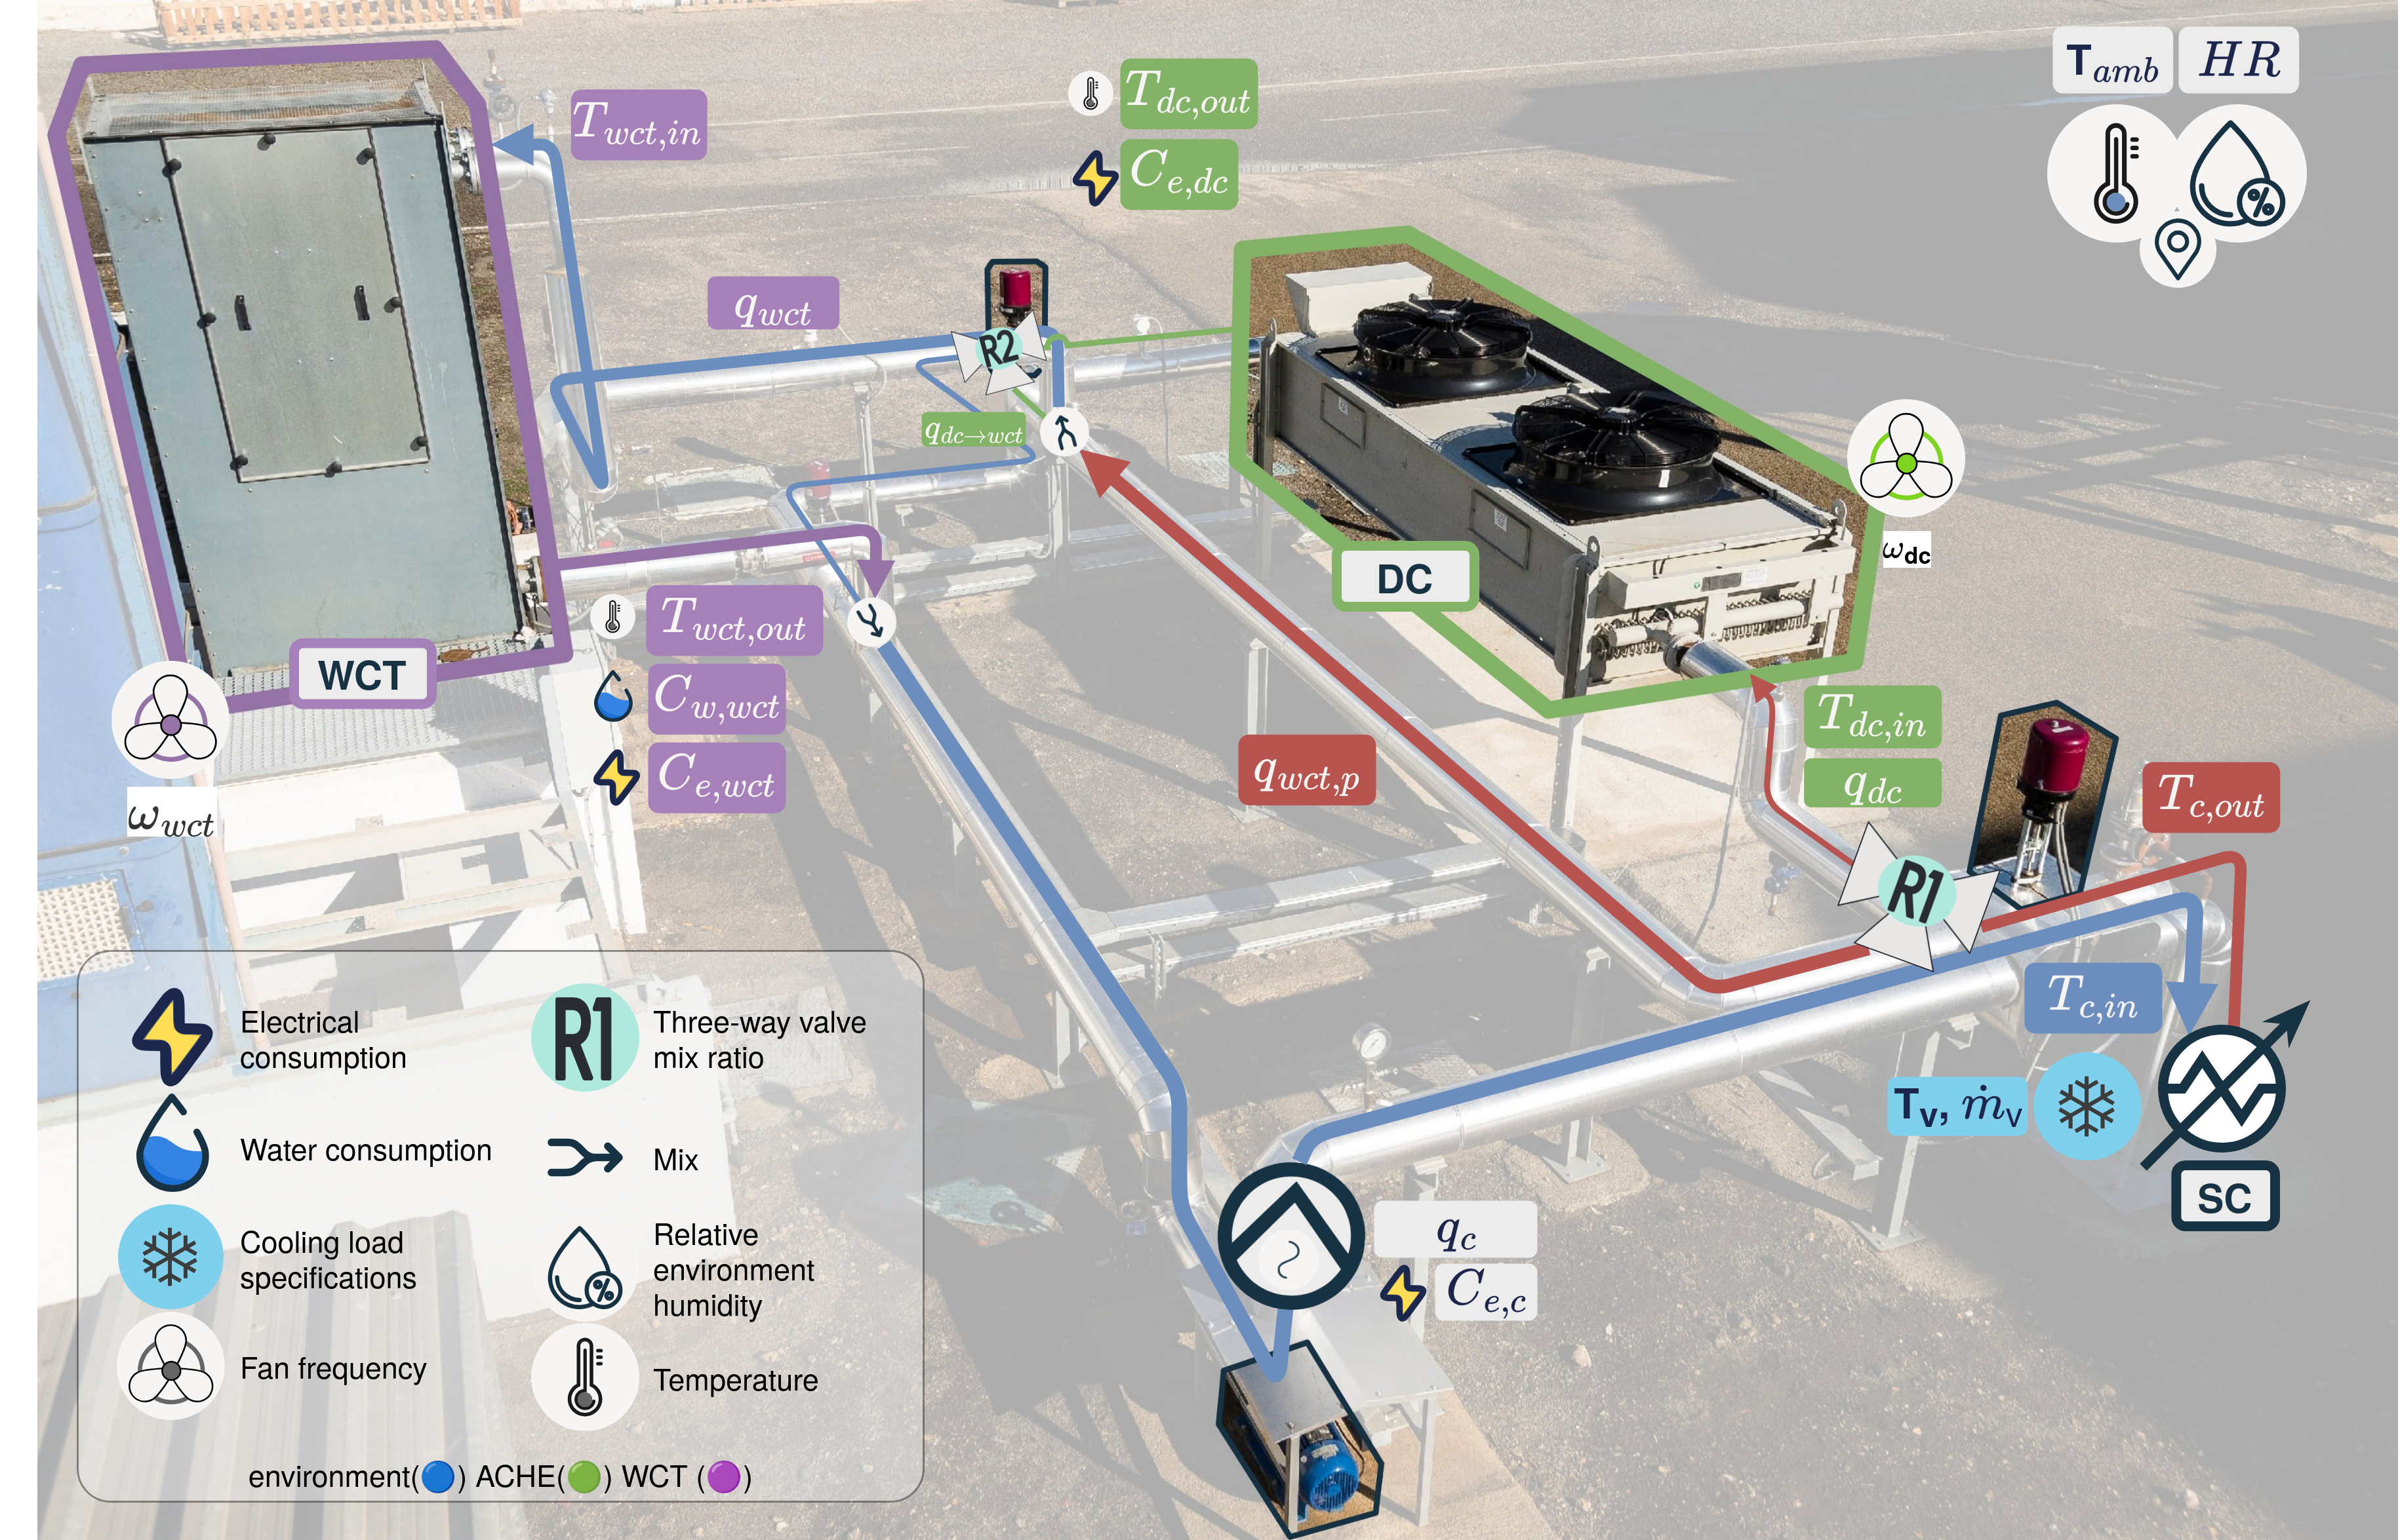
\includegraphics[width=.9\linewidth]{WASCOP-facility-diagram.png}
	\caption{\gls{psaLabel} combined cooling system facility}
	\labfig{cc:facility:cc-pilot-plant-diagram}
\end{figure*}


%===================================
%===================================
\section{Plant description}
\labsec{cc:facility:description}

% Sacado de: Wet cooling tower performance prediction in \gls{cspLabel} plants:
% A comparison between artificial neural networks and Poppe’s model
The pilot plant of combined cooling systems located at \gls{psaLabel} (see the
layout in \reffig{cc:facility:pid}) consists of three circuits: cooling,
exchange and heating. In the cooling circuit, water circulating inside the tube
bundle of a \fullgls{scLabel} (main design specifications in
\reftab{cc:facility:sc}) can be cooled through a \fullgls{wctLabel} and/or a
\fullgls{dcLabel} (type \gls{acheLabel}, characteristics available in
\reftab{cc:facility:dc}), both with a designed thermal power of
204~kW$_{\text{th}}$. In the exchange circuit, a saturated steam generator of
80~kW$_{\text{th}}$ (on the design point), generates steam at different
pressures (in the range between 82~mbar and 200~mbar), which is in turn
condensed in the surface condenser. In this way, the steam transfers its latent
heat of condensation to the refrigeration water, that is heated. Finally, in the
heating circuit, a solar field with a thermal power of 300~kW$_{\text{th}}$ at
the design point, provides the energy required by the steam generator, in the
form of hot water. It is a unique, very flexible, fully instrumented and
versatile facility, able to operate in different operation modes: series and
parallel mode, conventional dry-only mode (all water flow is cooled through the
dry cooling tower) and wet-only mode (all water flow is cooled through the wet
cooling tower).

The instrumentation related to the system components is described
in \reftab{cc:facility:instr}. 

\begin{marginfigure}[-7.4cm]
    \includegraphics[]{WASCOP-facility-WCT.png}
	\caption{Back view of the \gls{wctLabel}}
    \labfig{cc:facility:wct-back-view}
\end{marginfigure}

% With regard to operational aspects of the system, note that the cooling water
% and air flow rates at the experimental facility ($\dot{m}_{wct}$, and air,
% $\dot{m}_{wct,air}$, respectively), are modified with the \textit{Pump 1} and
% the fan frequency percentage \texttt{\gls{scLabel}-001}, respectively (see
% \reffig{cc:facility:pid}).

\begin{table}[h]
\caption[Characteristics of instrumentation]{Characteristics of instrumentation ($^a$~value of the temperature in $^\circ$C, $^b$~of reading, $^c$~full scale, $^d$~mean value).} 
\labtab{cc:facility:instr}
\resizebox{\textwidth}{!}{
\begin{tabular}{cccc} 
    \toprule
    \textbf{Measured variable} & \textbf{Instrument} & \textbf{Range}  &
    \textbf{Measurement uncertainty}\\
    \midrule
    Water temperature & Pt100 & 0--100~$^\circ$C & 0.03 + 0.005$\cdot T^a$\\
    (\texttt{TT-001}... \texttt{TT-007}) & & &\\
    Cooling water flow rate & Vortex flow meter & 9.8 - 25 m$^3$/h & $\pm$ 0.65
    \% o.r.$^b$\\
    (\texttt{FT-001}...\texttt{FT-003})  & & &\\
    Water flow rate  & Paddle wheel & 0.05--2~m$^3$/h & $\pm$ 0.5 \% of
    F.S$^c$  \\
    (\texttt{FT-004}) & flow meter  & & + 2.5 \% o.r\\
    Condensate water & Coriolis flow meter & 0.1--0.3 m$^3$/h & $<$ 0.1  \% \\
    flow rate  (\texttt{FT-006}) &   & & \\
    
    Ambient temperature & Pt1000 & -40 - 60 $^\circ$C  & $\pm$ 0.4 $@$20
    $^\circ$C \\
    Relative humidity & Capacitive sensor & 0--98~\% & $\pm$ 3~\% o.r $@$20
    $^\circ$C  \\
            Air velocity & Impeller anemometer & 0.1--15$~\mbox{m s$^{-1}$}$ &
            $\pm$ 0.1$~\mbox{m s$^{-1}$}$ + 1.5 \%  o.r \\
            Outlet air temperature & Pt100   & -20--70~$^\circ$C & $\pm$
            0.5~$^\circ$C \\
            Outlet air humidity & Capacitive sensor   & 0--100~\%& $\pm$ 2~\% \\
    \bottomrule
\end{tabular}
}
\end{table}

%===================================
%===================================
\section{Experimental campaigns}
\labsec{cc:facility:exp}

With the aim of characterizing and developing models for this novel facility
several experimental campaigns have been carried out over the years.

The normative framework followed to carry out the experiments, in order to
ensure stable conditions, has been the standards \texttt{UNE
13741}~\sidecite{une_thermal_2004a} and the Spanish
CTI~\sidecite{cti_code_2000}. These standards specify the test duration and the
allowed variations of the most representative ambient and operating magnitudes
(water flow rate, heat load, cooling tower range, wet-bulb and dry-bulb
temperatures and wind velocity) during the tests ---specific to \gls{wctLabel}
and extended to the other components. Although the duration of the test should
not be less than one hour according to the standards, due to the low capacity of
the components in the \gls{psaLabel} pilot plant and the operational experience, the
duration of the tests has been reduced to up to 30 minutes. Once stable
conditions are maintained during the defined interval time, the average and
deviations values of each measurement are calculated in order to check that they
are within the allowable limits of the norm, which finally lead to a valid
steady-state operating point. 

\begin{figure}
    \includegraphics[width=\textwidth]{WASCOP-facility-PID.png}
    \caption{Layout of combined cooling systems pilot plant at \gls{psaLabel}.}
    \labfig{cc:facility:pid}
\end{figure}

Specifically, 11 experimental campaigns have been conducted at the pilot plant,
which have been classified according to its goal. \reftab{cc:exp-campaigns}
summarizes these experimental campaigns, describing the \gls{doeLabel} employed
and indicating the number of tests conducted under steady-state conditions. The
ranges of the variables involved in the experiments are also indicated, with
those used to define the \gls{doeLabel} for each test campaign shown in bold.
    
% The data for the different experimental campaigns in the \gls{wctLabel} is
% available at~\sidecite[*-4]{palenzuela_steadystate_2024a,serrano_wet_2024}

%================================
\subsection{Physical model calibration campaigns}

\begin{margintable}[*-3]
    \centering
    \caption{Main characteristics of the \gls{acheLabel} dry cooler at the pilot plant}
    \labtab{cc:facility:dc}
    \resizebox{\linewidth}{!}{
    \begin{tabular}{lcc}
        \toprule
        \textbf{Concept} & \textbf{Value} & \textbf{Unit} \\
        \midrule
        Number of tubes ($n_{dc,tb}$) & 60 & - \\
        Number of passes per tube ($k_{dc,tb}$) & 3 & - \\
        Tube length ($L_{dc,tb}$) & 3.6 & m \\
        Outer tube diameter ($D_{dc,o}$) & 12.7 & mm \\
        Inner tube diameter ($D_{dc,i}$) & 9.4 & mm \\
        Tube material & Copper & - \\
        Fin thickness & 0.21 & mm \\
        Fin spacing & 2.4 & mm \\
        Fin material & Aluminum  & - \\
        \bottomrule
    \end{tabular}
    }
\end{margintable}

\begin{margintable}[*7] 
    \centering
    \caption{Main characteristics of the surface condenser at the pilot plant}
    \labtab{cc:facility:sc}
    \resizebox{\linewidth}{!}{
    \begin{tabular}{lcc}
        \toprule
        \textbf{Concept} & \textbf{Value} & \textbf{Unit} \\
        \midrule
        Number of tubes & 96 & - \\
        Number of passes per tube & 4 & - \\
        Tube length & 3 & m \\
        Outer tube diameter & 21.34 & mm \\
        Tube thickness & 2.108 & mm \\
        Thermal cond. of the tube wall & 50 & W/(m·K) \\
        Tube-side inlet pressure & 5 & bar \\
        Tube-side fouling & 1.72$\cdot 10^{-5}$ & $ \mathrm{m}^2 \cdot \mathrm{K} / \mathrm{W} $ \\
        \bottomrule
    \end{tabular}
    }
\end{margintable}

\begin{itemize}
    \item \textit{\gls{wctLabel}-fan}. The aim of this campaign was to fit a
        function (mapping) that relates the air mass flow rate at the outlet of
        the tower, $\dot{m}_{wct,air}$, with the frequency of the fan,
        $\omega_{wct}$. Air velocity and temperature were measured at 8
        different fan speed levels, ranging from 30~\% to 100~\% in 10~\%
        increments (see \reftab{cc:exp-campaigns} -- \textit{\gls{wctLabel}-fan}). 
        
        Sensors measuring the air velocity, temperature and relative humidity at
        the outlet area of the wet cooling tower are not permanently installed
        in the plant. Portable sensors were used instead in some experiments to
        characterize them. They were measured at the outlet area of the cooling
        tower ---using the sensors listed in \reftab{cc:facility:instr} and at
        the top of the tower in \reffig{cc:facility:wct-back-view}. The outlet
        area was divided into 9 quadrants and the above mentioned magnitudes
        were registered at the center of each quadrant. The obtained values were
        averaged to determine the mean velocity, temperature and relative
        humidity used in the air mass flow rate calculation.

        % The \gls{wctLabel} fan area was divided into six quadrants,
        % and measurements were taken at the center of each quadrant. The recorded
        % values were then averaged to obtain the mean air velocity and
        % temperature, which were used to calculate the air mass flow rate. 
    
    \item \textit{\gls{dcLabel}-fan}. The aim of this campaign was to fit a
        function (mapping) that relates the air mass flow rate at the outlet of
        the \gls{dcLabel}, $\dot{m}_{dc,air}$, with the frequency of the fan,
        $\omega_{dc}$ (see \reftab{cc:exp-campaigns} --
        \textit{\gls{dcLabel}-fan}). Air velocity and temperature were measured
        at 10 different fan speed levels, ranging from 11~\% to 100~\% in 10~\%
        increments. The \gls{acheLabel} fan area was divided into eight
        quadrants, and measurements were taken at the center of each quadrant.
        The recorded values were then averaged to obtain the mean air velocity
        and temperature, which were used to calculate the air mass flow rate.
    
    \item \textit{\gls{wctLabel}-cal}. The experimental campaign was designed to
        calibrate the physical model by focusing on the Merkel number, which
        depends on the water-to-air mass flow ratio\sidenote{Further explained
        in \refsec{cc:modelling:wct:physical}}.
        %  This enables the
        % calculation of the air mass flow rate at the outlet of the cooling
        % tower, $\dot{m}_{wct,air}$, using the permanent sensors installed in the
        % facility}. 
        % Tests were performed under consistent summer conditions, with
        % high ambient temperatures and low relative humidities.
    
    \item \textit{\gls{dcLabel}-cal}. An experimental campaign (\textit{\gls{dcLabel}-cal}) was designed and performed to calibrate the Nusselt
        number correlation as described in \refsec{cc:modelling:dc:physical}.
    
    \item \textit{SC-cal}. Designed to calibrate the global heat transfer
    coefficient, $U_{dc}$, as a function of inlet water temperature, $T_{c,in}$
    and water flow rate, $q_{dc}$.
\end{itemize}

    
%================================
\subsection{Data-driven models training campaigns}


The data required for data-driven models depends on several factors such as the
complexity of the model and the diversity of the inputs. With the aim of
obtaining reliable data-driven models, data collected over several years of
operation were used for model training. 
    
\textit{\gls{wctLabel}-tr} and \textit{\gls{dcLabel}-tr} refer to the data collected to tune the \gls{wctLabel}
and \gls{dcLabel} data-driven models, respectively.

%================================
\subsection{Models validation campaigns}

The experimental campaigns designed for the thermal model's calibration were
repeated to validate the models of \gls{wctLabel} (\textit{\gls{wctLabel}-val}), \gls{dcLabel}
(\textit{\gls{dcLabel}-val}) and SC (\textit{SC-val}). An additional experimental
campaign was designed and performed to validate the complete model of the CC
system (\textit{CC-val}).


\begin{table*}[]
\centering
\caption[Experimental campaigns performed at the \gls{ccLabel} pilot plant]{Experimental campaigns performed at the \gls{ccLabel} pilot plant, where GD-n$_1$-n$_2$ refers to the spatial grid distribution ($n_1$) around the fan with $n_2$ measurements in each quadrant (\textit{$n_1 \times n_2$} measurements); \textit{BB-$n_1$-$n_2$} denotes a Box-Behnken design with \textit{$n_1$} variables and \textit{$n_2$} levels; and \textit{FF-$n_1$-...-$n_i$} indicates a full factorial design with \textit{$i$} variables, each with \textit{$n_i$} levels.}
\labtab{cc:exp-campaigns}
\resizebox{\linewidth}{!}{%
\begin{tabular}{rlclclccccccclclclccccc}
\hline
\multirow{2}{*}{\textbf{Features}}                               &                      & \multicolumn{9}{c}{\textbf{Physical model calibration}}                                                                                                                                         & \multicolumn{1}{l}{} & \multicolumn{3}{c}{\textbf{Data-driven models training}}    &                      & \multicolumn{7}{c}{\textbf{Validation}}                                                                                                              \\ \cline{3-11} \cline{13-15} \cline{17-23} 
                                                        &                      & \gls{wctLabel}-fan &                      & \gls{wctLabel}-cal &                      & \gls{dcLabel}-fan & \multicolumn{1}{l}{} & \gls{dcLabel}-cal & \multicolumn{1}{l}{} & \gls{scLabel}-cal & \multicolumn{1}{l}{} & \gls{wctLabel}-tr &                      & \gls{dcLabel}-tr &                      & \gls{wctLabel}-val &                      & \gls{dcLabel}-val & \multicolumn{1}{l}{} & \gls{scLabel}-val & \multicolumn{1}{l}{} & \gls{ccLabel}-val  \\ \cline{1-1} \cline{3-3} \cline{5-5} \cline{7-7} \cline{9-9} \cline{11-11} \cline{13-13} \cline{15-15} \cline{17-17} \cline{19-19} \cline{21-21} \cline{23-23} 
\gls{doeLabel}                                          &                      & GD-6-8             &                      & FF-2-2-2-2         &                      & GD-8-10           & \multicolumn{1}{l}{} & BB-4-3            & \multicolumn{1}{l}{} & BB-3-3            & \multicolumn{1}{l}{} & -                 &                      & -                &                      & FF-2-2-2-2         &                      & BB-4-3            & \multicolumn{1}{l}{} & BB-3-3            & \multicolumn{1}{l}{} & FF-2-2-2-3         \\
$N_{tests}$                                             &                      &
48                 &                      & 17                 &
& 80                & \multicolumn{1}{l}{} & 27                &
\multicolumn{1}{l}{} & 15                & \multicolumn{1}{l}{} & 115
&                      & 137              &                      & 17
&                      & 27                & \multicolumn{1}{l}{} & 15
& \multicolumn{1}{l}{} & 24                 \\
$T_{amb}$ ($^\circ$C)                                   &                      & 20-23              &                      & 31-41              &                      & 26                &                      & \textbf{12 - 29}  &                      & -                 &                      & 9-39              &                      & 9-39             &                      & 15-29              &                      & \textbf{13 - 32}  &                      & -                 &                      & \textbf{12 - 37}   \\
HR (\%)                                                 &                      & -                  &                      & 13-40              &                      & -                 &                      & -                 &                      & -                 &                      & 10-87             &                      & -                &                      & 15-29              &                      & -                 &                      & -                 &                      & 14 - 63            \\
$\dot{m}_v$ (kg/h)                                      &                      & -                  &                      & -                  &                      & -                 &                      & -                 &                      & 118 - 328         &                      & -                 &                      & -                &                      & -                  &                      & -                 &                      & 133 - 287         &                      & 200 - 310          \\
$\dot{Q}_c$ (kW)                                        &                      & -                  &                      & -                  &                      & -                 &                      & -                 &                      & \textbf{78 - 216} &                      & -                 &                      & -                &                      & -                  &                      & -                 &                      & \textbf{88 - 187} &                      & \textbf{132 - 202} \\
$q_{c}$ (m$^3$/h)                                       &                      & -                  &                      & -                  &                      & -                 &                      & -                 &                      & \textbf{10 - 24}  &                      & -                 &                      & -                &                      & -                  &                      & -                 &                      & \textbf{10 - 24}  &                      & \textbf{18 - 24}   \\
$q_{dc}$ (m$^3$/h)                                      &                      & -                  &                      & -                  &                      & -                 &                      & \textbf{5 - 25}   &                      & -                 &                      & -                 &                      & 5-24             &                      & -                  &                      & \textbf{5 - 24}   &                      & -                 &                      & \textbf{5 - 24}    \\
$q_{wct}$ (m$^3$/h)                                     &                      & -                  &                      & 8-22               &                      & -                 &                      & -                 &                      & -                 &                      & 6-23              &                      & -                &                      & 6-22               &                      & -                 &                      & -                 &                      & \textbf{6 - 24}    \\
$T_{dc,in}$ ($^\circ$C)                                 &                      & -                  &                      & -                  &                      & -                 &                      & \textbf{35 - 41}  &                      & -                 &                      & -                 &                      & 31-54            &                      & -                  &                      & \textbf{31 -42}   &                      & -                 &                      & 33 - 54            \\
$\Delta T_{dc,in-out}$ ($^\circ$C)                      &                      & -                  &                      & -                  &                      & -                 &                      & \textbf{2 - 7}    &                      & -                 &                      & -                 &                      & 1-13             &                      & -                  &                      & \textbf{2 - 9}    &                      & -                 &                      & 1 - 11             \\
$T_{v}$ ($^\circ$C)                                     &                      & -                  &                      & -                  &                      & -                 &                      & -                 &                      & \textbf{36 - 56}  &                      & -                 &                      & -                &                      & -                  &                      & -                 &                      & \textbf{36 - 56}  &                      & \textbf{36 - 57}   \\
$T_{wct,in}$ ($^\circ$C)                                &                      & -                  &                      & 31-49              &                      & -                 &                      & -                 &                      & -                 &                      & 33-41             &                      & -                &                      & 35-40              &                      & -                 &                      & -                 &                      & 33 - 54            \\
\multicolumn{1}{c}{$\Delta T_{wct,in-out}$ ($^\circ$C)} & \multicolumn{1}{c}{} & -                  & \multicolumn{1}{c}{} & 6-18               & \multicolumn{1}{c}{} & -                 &                      & -                 &                      & -                 &                      & 2-16              & \multicolumn{1}{c}{} & -                & \multicolumn{1}{c}{} & 4-11               & \multicolumn{1}{c}{} & -                 &                      & -                 &                      & 4-11               \\
$\omega_{dc}$ (\%)                                      &                      & -                  &                      & -                  &                      & 11 - 100          &                      & \textbf{11 - 76}  &                      & -                 &                      & -                 &                      & 11-100           &                      & -                  &                      & \textbf{11 - 98}  &                      & -                 &                      & 11 - 100           \\
$\omega_{wct}$ (\%)                                     &                      & 30-100             &                      & 25-100             &                      & -                 &                      & -                 &                      & -                 &                      & 21-93             &                      & -                &                      & 21-48              &                      & -                 &                      & -                 &                      & 21 - 87            \\ \hline
\end{tabular}%
}
\end{table*}


% %===================================
% \subsection{Data-driven models training -- Exp 2}[Exp 2] 
% \labsec{cc:facility:exp:2}


% %===================================
% \subsection[Experimental campaign 3]{Validation -- Exp 3}[Exp 3] 
% \labsec{cc:facility:exp:3}

% With the aim of validating and comparing different modelling approaches, a
% dataset of 17 tests (different from the ones taken for experimental campaigns 1
% and 2) has been compiled. This experimental campaign was designed using a
% design of experiments based on full factorial design with 4 factors and 2
% levels (low and high), whose values are shown in
% \reftab{cc:facility:exp:3:doe}.  

% \begin{margintable}[*-5]
%     \caption{Design of experiments for model comparison (Exp 3)} 
%     \labtab{cc:facility:exp:3:doe} 
%     \resizebox{\linewidth}{!}{
%     \begin{tabular}{cccc} 
%         \toprule Variable & Low level & High level  \\
%         \midrule $T_{wb}$ ($^{\circ}$C) & $\leq$ 10 & $\geq$ 15 \\
%         $T_{wct,in}$ ($^{\circ}$C) & $\leq$ 37 & $\geq$ 39 \\
%         $\dot{m}_{wct}$ (kg/s) & $\leq$ 3.3 & $\geq$ 5 \\
%         $T_{wct,in}-T_{wct,out}$ ($^{\circ}$C)  & $\leq$ 7 & $\geq$ 8 \\
%         \bottomrule 
%     \end{tabular}
%     }
% \end{margintable}

% % An additional test at design operating conditions of the \gls{wctLabel}
% % (\mbox{$T_{b,\infty}$=21 $^{\circ}$C}, $T_{w,i}$=40 $^{\circ}$C,
% % $\dot{m}_w$=6.9 kg/s and $T_{w,i}-T_{w,o}$=7 $^{\circ}$C) has been also
% % included in this test campaign, where $T_{b,\infty}$ is the ambient wet bulb
% % temperature and $T_{w,o}$ the temperature of the water at the outlet of the
% % \gls{wctLabel}. 


% %===================================
% %===================================
% \subsection{Dry cooler, Surface condenser and Combined cooler models}
% \labsec{cc:facility:exp-others}

% \reftab{cc:exp-campaigns} summarizes the experimental campaigns,
% describing the \gls{doeLabel} employed and indicating the number of
% tests conducted under steady-state conditions. The ranges of the variables
% involved in the experiments are also indicated, with those used to define the
% \gls{doeLabel} for each test campaign shown in bold.


% %================================
% \subsubsection{Complete system validation -- CC-val}
% \labsec{cc:facility:exp:cc}

% An additional experimental campaign (\reftab{cc:exp-campaigns} --
% \textit{CC-val}) was designed and performed to validate the complete model of
% the \gls{ccLabel} system. This campaign comprises 24 tests.       

